\subsection*{Simuleringer}
Efter at indgangsvælgeren er blevet designet og beregnet, er der lavet en række simuleringer for se om kredsløbet opfører sig som ønsket og, hvis der er afvigelser, give en begrundelse for hvorfor. I dette afsnit vil der blive simuleret følgende, Dæmpning af signal, THD, frekvenskarakteristik, forstærkning i kredsløbet, tænd og sluk af signal. Det samlede diagram der er simuleret kan ses på figur \ref{diagram_simulering}. 

\begin{figure}[h]
\centering
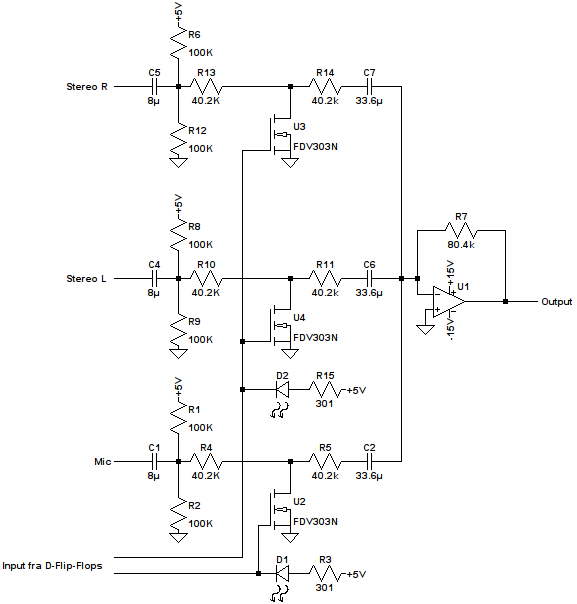
\includegraphics[width=\textwidth]{teknisk/indgangsvaelger/simulering/indgangvaelger_ltspice_diagram.png}
\caption{Diagram over det kredsløb der simuleres.}
\label{diagram_simulering}
\end{figure}

\subsubsection*{Forstærkning i kredsløbet}
Fra beregningerne vides det at kredsløbet er designet til at have en forstærkning på 1. Derudover vil signalet efter indgangsvælgeren også være inverteret fordi der bruges en inverterende forstærker til at sumerer signalerne. Det simulerede signal er vist på figur \ref{indgangsvaelger_input/output}. Simuleringen er lavet ved en transient analyse over 3 ms, med en maksimum timestep på 0,01 µs og 2 V peak 1kHz på indgangen. På figur \ref{indgangsvaelger_input/output} ses det at forstærkningen på 1 opnået og signalet er inverteret som forventet. Signalet er ikke helt 2 V peak, det skyldes at generatoren har en udgangsmodstand på 2,2 k\ohm.
\begin{figure}[h]
\centering
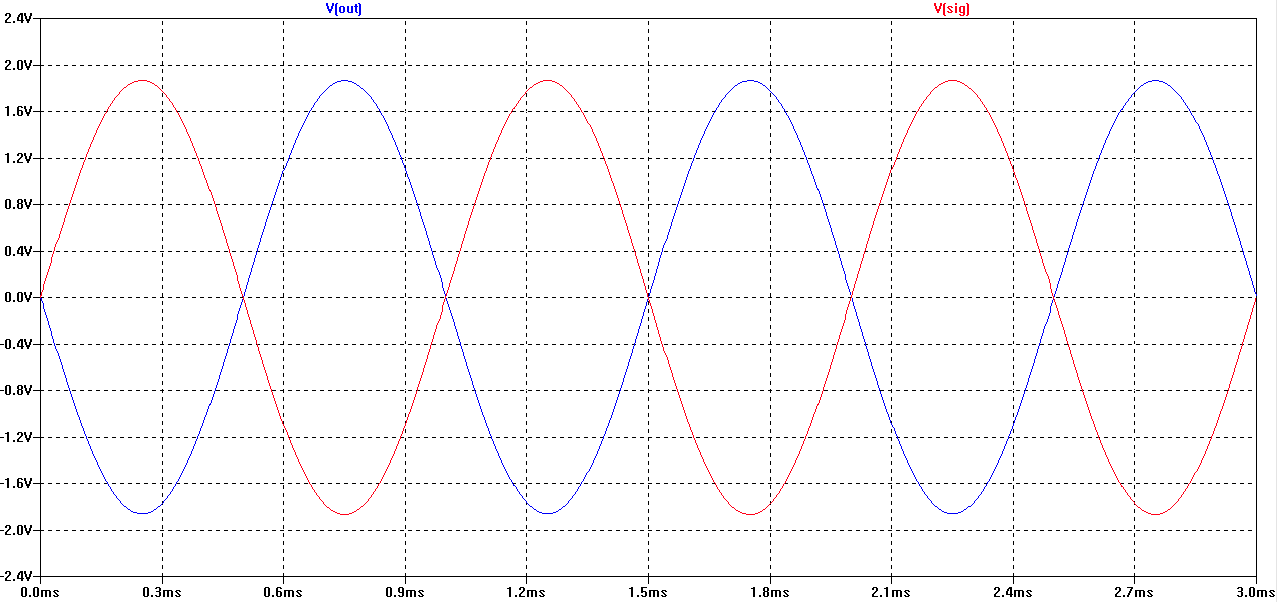
\includegraphics[width=\textwidth]{teknisk/indgangsvaelger/simulering/input_output.png}
\caption{Forstærkningen igennem indgangsvælgeren. Den røde kurve inputsignalet til indgangsvælgeren og den blå er outputsignalet fra indgangsvælgeren.}
\label{indgangsvaelger_input/output}
\end{figure}

\subsubsection*{Frekvenskarakteristik}
På figur \ref{indgangsvaelger_frekvenskarakteristik} er simuleringen af frekvenskarakteristikken vist. Simuleringen er lavet ved en AC-Analyse fra 2 Hz til 200 kHz, og ved at sætte output over input ved en 0 V på transistoren. Fra kravspecifikation er der opsat krav om at i frekvensområdet fra 20 Hz til 20 kHz må afvigelsen højest være $\pm$ 1,5 dB. På simuleringen ses det at fra 10 kHz til 20 kHz er der en lille afvigelse på ca. 0,06 dB. Afvigelsen skyldes at transistoren der er brugt har en passiv kapacitet, der gør at ved høje frekvenser vil signalet falde af.

\begin{figure}[h]
\centering
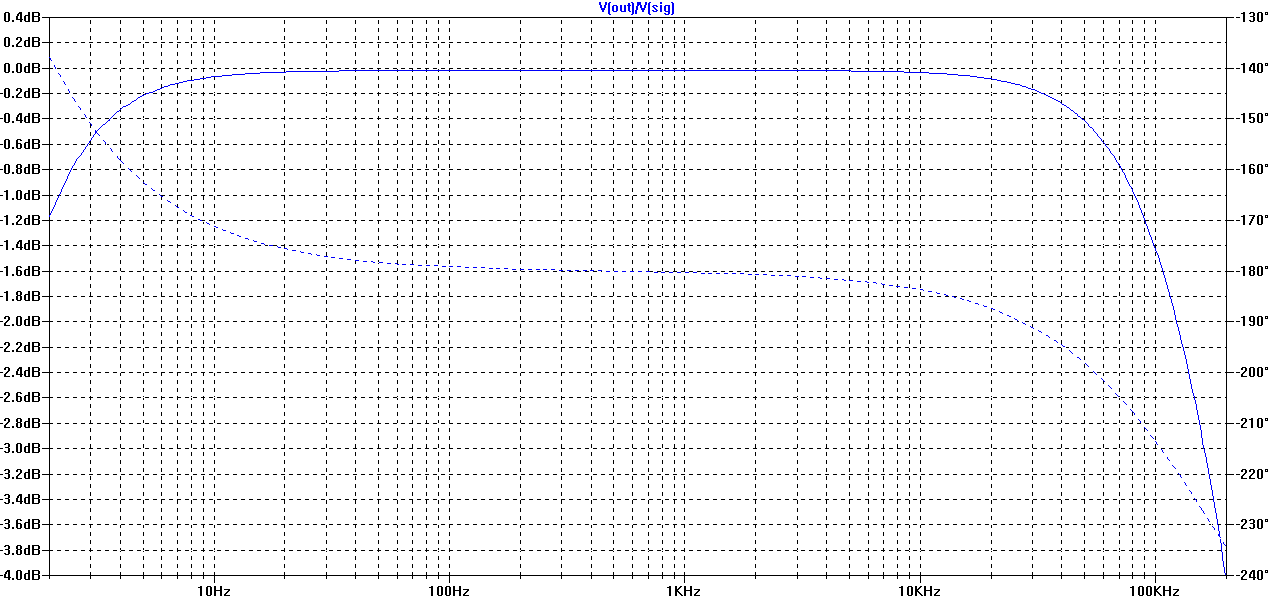
\includegraphics[width=\textwidth]{teknisk/indgangsvaelger/simulering/frekvenskarakteristik.png}
\caption{Frekvens- og fasekarakteristikken for indgangsvælgeren.}
\label{indgangsvaelger_frekvenskarakteristik}
\end{figure}

\subsubsection*{Dæmpning af signal}
På figur \ref{indgangsvaelger_daempniing} ses en graf over hvor stor en dæmpning er simuleret til i kredsløbet. Simuleringen er lavet ved en AC-Analyse fra 2 Hz til 200 kHz, og ved at sætte output over input ved en 5 V på transistoren. Fra kravspecifikationen er der opsat krav om at isoleringen af signaler skal være større end 50 dB. Dæmpningen er aflæst til minimum 89 dB.
\begin{figure}[h]
\centering
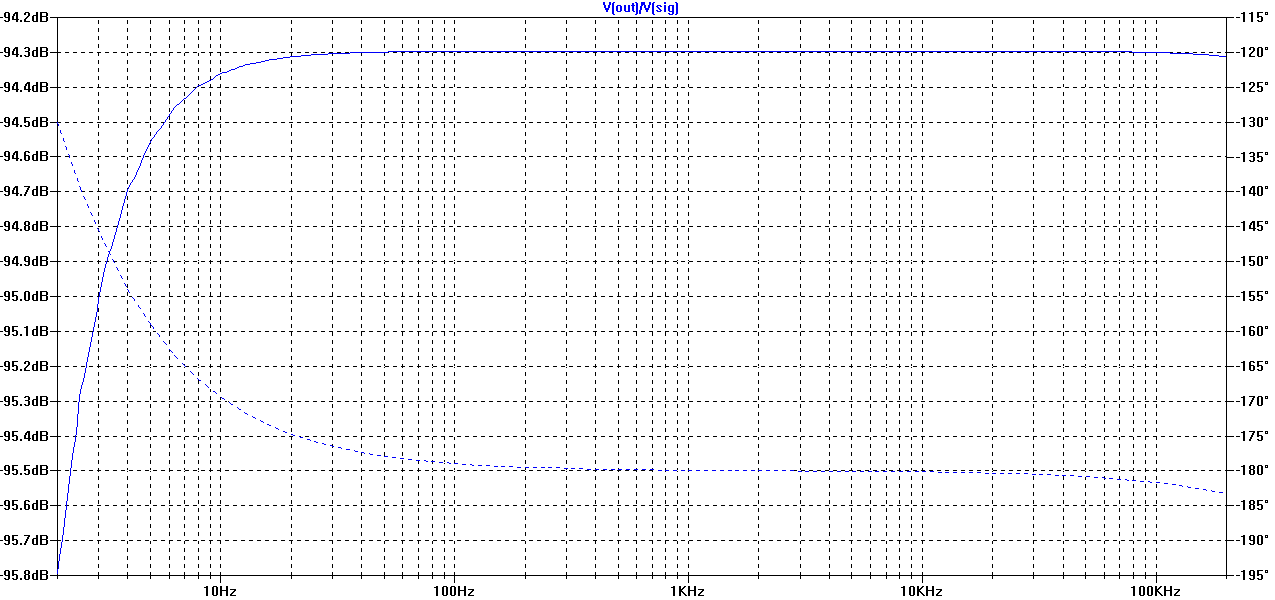
\includegraphics[width=\textwidth]{teknisk/indgangsvaelger/simulering/daempning_af_signal.png}
\caption{Dæmpningsgraden af signalet, når det er slukket.}
\label{indgangsvaelger_daempniing}
\end{figure}

\subsubsection*{Tænd og sluk af signal}
På figur \ref{indgangsvaelger_taendsluk} er der simuleret at en signal bliver tændt og slukket. Simuleringen er lavet ved en transient analyse over 1,4 s, med en maksimum timestep på 0,1 µs og 2 V peak 100 Hz på indgangen. Først er signalet slukket i 100 ms, dernæst er signalet tændt i 700 ms og til sidst er signalet slukket i 600 ms. Som det ses er signalet når det bliver tændt først oppe på niveau efter det har været tændt i 700 ms. Det skyldes at der er brugt kondensatorer i kredsløbet, hvilket giver en længere indsvingningstid.
\begin{figure}[h]
\centering
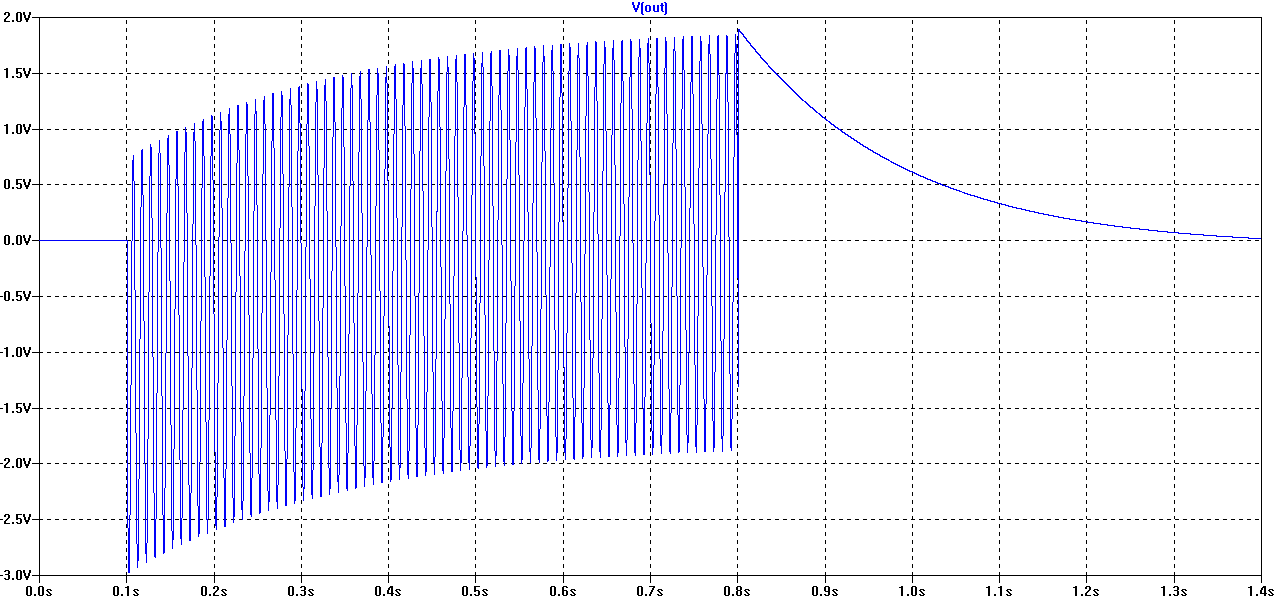
\includegraphics[width=\textwidth]{teknisk/indgangsvaelger/simulering/taend_sluk.png}
\caption{Simulering af at tænde og slukke signalet.}
\label{indgangsvaelger_taendsluk}
\end{figure}

\textbf{THD}
\newline
Simuleringen er lavet ved en fourier-analyse, og giver en THD på 0.062\%.
